\documentclass[12pt]{article}

\usepackage{listings}
\usepackage{graphicx}

\lstset{
  basicstyle=\small,
  breaklines=true
  }


\date{\today}
\title{ECOTE - preliminary project \\ 
Translator of a \LaTeX \, subset to HTML
}
\author{Krzysztof Rudnicki, 307585 \\
Semester: 2023L}

\begin{document}
\maketitle
\section{General overview and assumptions}
My task is to create a translator of \LaTeX \, subset to selected text format with focus on \LaTeX \, tables \\ 
I decided to change to translator of \LaTeX \, subset to HTML since I know \LaTeX \, very well and HTML relatively well, I decide to translate \LaTeX into HTML since HTML is easy, a little bit different than \LaTeX and popular which makes this translator a practical tool.
\subsection{Assumptions}
\begin{itemize}
    \item No \LaTeX \, (\%) comments in the script 
    \item There are no extra packages in \LaTeX \, script (provided with \\ \textbackslash usepackage keyword) besides ones distributed with \LaTeX
    \item There are no extra classes in \LaTeX \, script besides ones distributed with \LaTeX
    \item There is nothing between \textbackslash documentclass keyword and \\ \textbackslash begin\{document\} keyword 
    \item No standard \LaTeX \, instructions are modified in the script
    \item "Tables" will be represented using \LaTeX \, \emph{table} environment 
\end{itemize}
\section{Functional requirements}
The goal of the project is to transform .tex file to (working ) .html file if the subset of .tex file is within project scope or output error message explaining why the html could not be outputed
\subsection{\LaTeX \, subset}
This project will focus almost exclusively on \emph{tabular} environment \\
\begin{itemize}
    \item $\backslash$documentclass\{class\}: Defines what layout standard \LaTeX will use 
    \item $\backslash$begin\{document\}: Ends (in our case empty) preamble
    \item $\backslash$end\{document\}: Ends \LaTeX \, document
    \item $\backslash$begin\{tabular\}[pos]\{table spec\}: Opens environment used to typeset tables 
    \item $\backslash$end\{tabular\}: Closes environment used to typeset tables 
\end{itemize}
Supported tabular arguments:
\begin{itemize}
    \item l, c, r - respectively left-justified, centered and right-justified column
    \item  | - single vertical line 
    \item  || - double vertical line 
    \item p\{'width'\} - paragraph column (that wraps), aligned at the top 
    \item m\{'width'\} - paragraph column (that wraps), aligned at the middle 
    \item b\{'width'\} - paragraph column (that wraps), aligned at the bottom 
\end{itemize}

Supported commands inside tabular environment
\begin{itemize}
    \item \& - separate columns
    \item $\backslash$$\backslash$ - start new row
    \item $\backslash$hline - horizontal line
    \item $\backslash$cline\{i-j\} horizontal line beginning in column i and ending in column j
    \item $\backslash$newline - new line \emph{inside} the cell
\end{itemize}
\section{Implementation}
I decided to use Python as a language in which I will implement my solution \\ 
The reasons for using python are as follow:
\begin{enumerate}
    \item It is the easiest language among those that I know
    \item I know it enough to be confident in my ability to implement this solution in python
    \item I want to learn python more through this project
\end{enumerate}
Negative aspects of python which is that it is very slow language do not bother me as I believe the project scope will not be big enough for this to become an issue
  
\subsection{General architecture}
\begin{tabular}{|l|p{10cm}|}
    \hline 
    Module & Description \\ 
    \hline 
    Main & Handles parameters inputed as program arguments and interaction between modules \\
    \hline
    FileHandler & Handles file reading \\ 
    \hline 
    LatexHandler & reads \LaTeX \, file content, parses it using LatexWalker class of pylatexenc library and detects errors \\
    \hline
    TabHandler & Transforms tabular environment into html table
    \\
    \hline
    TabArgHandler & Handles positional and table spec arguments of tabular environment and translates them to html \\ 
    \hline
    TabInsideHandler & Handles actual content of table and translates them to html \\
    \hline
    HTMLOutput class &  Transforms \LaTeX \, code into html with the assumptions that no errors were found by LatexHandler and if there were any they were dealt with \\ 
    \hline
\end{tabular}


\begin{figure}[h]
    \caption{Module class diagram}
    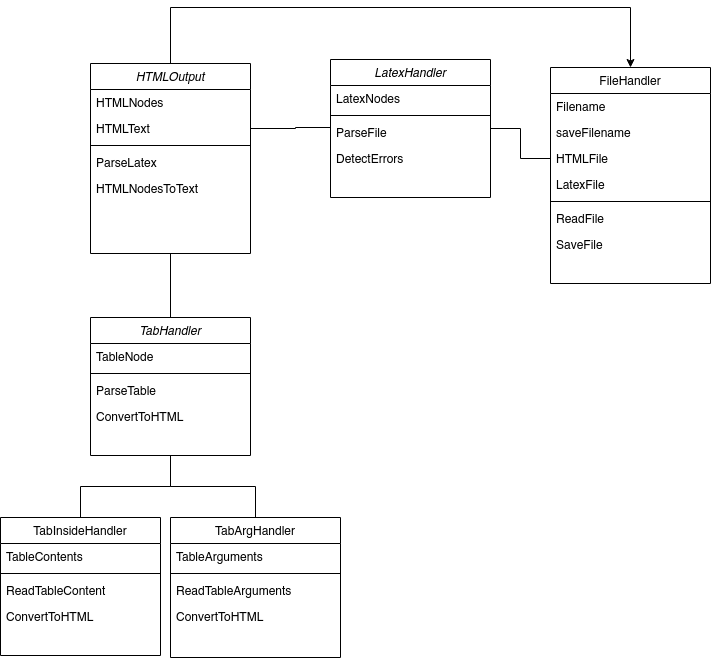
\includegraphics[width=\textwidth]{class.png}
\end{figure}
    





\subsection{Data structures}
\begin{itemize}
\item File entered by user is represented by python File class 
\item Parsed \LaTeX \, code is represented by data structure based on node classes 
\item Tabular environment parameters are stored in an array, if the parameter contains additional optional parameters they are stored in a pair of the parent argument and array of all optional arguments 
\item Generated HTML code is stored in node classes 
\item Final HTML code is stored in plain text and then written to File
\end{itemize}

\subsection{Module descriptions}
\subsubsection{Main}
Handles user arguments and communication between modules \\ 
Input: \\ 
args[] - Array of user inputed arguments \\ 
Functions: 
\begin{itemize}
    \item Handle arguments - Checks if arguments are correct and adjust program to their contents, in particular saves tex file path
    \item Invoke FileHandler - starts file handler class and gets returned file or errors 
    \item Invoke Latex Handler - Sends file from file handler to LatexHandler 
\end{itemize}
\subsubsection{FileHandler}
Reads file from filename provided by user and at the end saves HTML file \\ 
Parameters: \\ 
\begin{itemize}
\item filename - user entered tex filename
\item saveFilename - (optional) filename for output file 
\item HTMLFile - converted final html file in File format 
\item LatexFile - latex file in File format 
\end{itemize}
Functions: 
\begin{itemize}
    \item ReadFile - Using user filename as argument reads file and saves it to LatexFile
    \item SaveFile - Using filename provided by user or tex filename as argument converts HTML string to file and saves it 
\end{itemize}

\subsubsection{LatexHandler}
Reads file from filename provided by user and at the end saves HTML file \\ 
Parameters: \\ 
\begin{itemize}
\item filename - user entered tex filename
\item saveFilename - (optional) filename for output file 
\item HTMLFile - converted final html file in File format 
\item LatexFile - latex file in File format 
\end{itemize}
Functions: 
\begin{itemize}
    \item ReadFile - Using user filename as argument reads file and saves it to LatexFile
    \item SaveFile - Using filename provided by user or tex filename as argument converts HTML string to file and saves it 
\end{itemize}

\subsubsection{HTMLOutput}
Reads file from filename provided by user and at the end saves HTML file \\ 
Parameters: \\ 
\begin{itemize}
\item filename - user entered tex filename
\item saveFilename - (optional) filename for output file 
\item HTMLFile - converted final html file in File format 
\item LatexFile - latex file in File format 
\end{itemize}
Functions: 
\begin{itemize}
    \item ReadFile - Using user filename as argument reads file and saves it to LatexFile
    \item SaveFile - Using filename provided by user or tex filename as argument converts HTML string to file and saves it 
\end{itemize}

\subsubsection{TabHandler}
Handles tables and converts them to html nodes \\ 
Parameters: \\ 
\begin{itemize}
\item TableNode - node containing only the table
\end{itemize}
Functions: 
\begin{itemize}
    \item ParseTable - Parses Table node and checks for errors
    \item ConvertToHTML - Converts table node to html using TabInsideHandler and TabArgHandler
\end{itemize}

\subsubsection{TabInsideHandler}
Handles inside of tabular environment and converts them to html nodes  \\ 
Parameters: \\ 
\begin{itemize}
\item TableContents - Latex node containing only inside of table
\end{itemize}
Functions: 
\begin{itemize}
    \item ReadTableContent - Parses table content and checks for errors 
    \item ConvertToHTML - Converts table inside node to html
\end{itemize}

\subsubsection{TabArgHandler}
Handles arguments of tabular environment and converts them to html nodes  \\ 
Parameters: \\ 
\begin{itemize}
\item TableArguments - Arguments provided with $\backslash$begin\{tabular\} environment
\end{itemize}
Functions: 
\begin{itemize}
    \item ReadTableARguments - Parses table arguments and checks for errors 
    \item ConvertToHTML - Converts table arguments to html
\end{itemize}

\subsection{Input/output description}
Input is a .tex file (\LaTeX \, file) \\ 
Outpus is an .html file \\ 
In case of errors error message will be outputed on the terminal \\
Input File path is entered as an argument to terminal with "-i" or "--input" flag for example:
\begin{lstlisting}[language=bash]
python main.py -i texFile.tex
\end{lstlisting}
Output file path can be named by user by using "-o" or "--output" flag:
\begin{lstlisting}[language=bash]
python main.py -i texFile.tex -o htmlFile.html
\end{lstlisting}
If no "-o" flag is issued the output file will have the same name as input file with changed extension to html (so in this example texFile.tex will become texFile.html) \\ 
If the path to file name consists of spaces, path name needs to be but in ""
\begin{lstlisting}[language=bash]
python main.py -i "My Folder/input.tex"
\end{lstlisting}
\subsection{Others}
\section{Functional test cases}

\begin{tabular}{|p{3cm}|p{6cm}|p{6cm}|}
    \hline 
    Title  &  Input (\LaTeX) & Output \\
    \hline

    empty file &
    \begin{lstlisting}

    \end{lstlisting}&
    \begin{lstlisting}
Error! expected \documentclass at the begining of LaTeX file 
    \end{lstlisting} \\
    \hline

    Document class &
    \begin{lstlisting}
\documentclass[options]{class}
    \end{lstlisting}&
    \begin{lstlisting}
Error! expected \begin{document} after document class
    \end{lstlisting} \\
    \hline

    \begin{lstlisting}
Extra text between document class and begin document
    \end{lstlisting}&
    \begin{lstlisting}
\documentclass[options]{class}
"extra text"
\begin{document}
    \end{lstlisting}&
    \begin{lstlisting}
Error! unexpected text between document class and begin document
    \end{lstlisting}  \\
    \hline 

\begin{lstlisting}
Just document class and begin document
\end{lstlisting}&
\begin{lstlisting}
\documentclass[options]{class}
\begin{document}
\end{lstlisting}&
\begin{lstlisting}
Error! no \end{document} at the end of LaTeX code
\end{lstlisting}  \\
\hline 

    \end{tabular} 

\begin{tabular}{|p{3cm}|p{6cm}|p{6cm}|}
\hline 
Title  &  Input (\LaTeX) & Output \\
\hline

\begin{lstlisting}
Just document class and begin/end document
\end{lstlisting}&
\begin{lstlisting}
\documentclass[options]{class}
\begin{document}
\end{document}
\end{lstlisting}&
\begin{lstlisting}
<html>
</html>
\end{lstlisting}  \\
\hline 

\begin{lstlisting}
Plain text inside
\end{lstlisting}&
\begin{lstlisting}
\documentclass[options]{class}
\begin{document}
Lorem ipsum dolor sit amet.
\end{document}
\end{lstlisting}&
\begin{lstlisting}
<html>
Lorem ipsum dolor sit amet.
</html>
\end{lstlisting}  \\
\hline 

\begin{lstlisting}
Reduntant \end{document} (ignored)
\end{lstlisting}&
\begin{lstlisting}
\documentclass[options]{class}
\begin{document}
Lorem ipsum dolor sit amet.
\end{document}
\end{document}
\end{lstlisting}&
\begin{lstlisting}
<html>
Lorem ipsum dolor sit amet.
</html>
\end{lstlisting}  \\
\hline 

\begin{lstlisting}
LaTeX comments
\end{lstlisting}&
\begin{lstlisting}
\documentclass[options]{class}
\begin{document}
Lorem ipsum dolor sit amet.
% some comment
\end{document}
\end{document}
\end{lstlisting}&
\begin{lstlisting}
Error! LaTeX comment detected at line 3
\end{lstlisting}  \\
\hline 



\end{tabular}

\begin{tabular}{|p{3cm}|p{6cm}|p{6cm}|}
    \hline
Title  &  Input (\LaTeX) & Output \\
\hline

\begin{lstlisting}
Table with vertical lines
\end{lstlisting}&
\begin{lstlisting}
\documentclass[options]{class}
\begin{document}
\begin{tabular}{ l | c | r }
test & 2 & test \\
4 & 5 & 6 \\
\end{tabular}
\end{document}
\end{lstlisting}&
\begin{lstlisting}
<html>
<table>
<tr>
<td align='left'>test</td>
<td align='center' style="border-left: 1px solid black;">2</td>
<td align='right'>test</td>
</tr>
<tr>
<td align='left'>4</td>
<td align='center' style="border-left: 1px solid black;">5</td>
<td align='right'>6</td>
</tr>
</table>
</html>
\end{lstlisting}  \\
\hline 

\begin{lstlisting}
Missing &
\end{lstlisting}&
\begin{lstlisting}
\documentclass[options]{class}
\begin{document}
\begin{tabular}{ l c r }
1 & 2 & 3 \\
4 & 5 6 \\
\end{tabular}
\end{document}
\end{lstlisting}&
\begin{lstlisting}
Error! Missing third column in second row 
\end{lstlisting}  \\
\hline 

\end{tabular}

\begin{tabular}{|p{3cm}|p{6cm}|p{6cm}|}
    \hline
Title  &  Input (\LaTeX) & Output \\
\hline

\begin{lstlisting}
Too much columns
\end{lstlisting}&
\begin{lstlisting}
\documentclass[options]{class}
\begin{document}
\begin{tabular}{ l c r }
1 & 2 & 3 & 4 & 5 \\
4 & 5 6 \\
\end{tabular}
\end{document}
\end{lstlisting}&
\begin{lstlisting}
Error! Too much columns in row 1, expected 3, got 5
\end{lstlisting}  \\
\hline 

\end{tabular}
    
\end{document}